\documentclass[pageno]{jpaper}

\newcommand{\IWreport}{Spring 2019}
\newcommand{\quotes}[1]{``#1''}


\widowpenalty=9999

\usepackage{graphicx}
\usepackage[normalem]{ulem}
\useunder{\uline}{\ul}{}
\graphicspath{ {./../Analysis/} }
\begin{document}

\title{Measuring Musical Sampling Impact Through Network Analysis}

\author{Justin Tran\\Adviser: Andrea LaPaugh}

\date{}
\maketitle

\thispagestyle{empty}
\doublespacing
\begin{abstract}
Musical sampling influence has only recently been studied through network structures through the basic analysis of artist-artist sampling relationships. In this paper, I integrate the use of additional properties of music sampling (such as genre, time period, and audio element sampled) to investigate patterns of influence in the musical community at large. Using the WhoSampled dataset, I investigate statistical metrics such as the most-sampled artists songs as well as the trend for musical sampling over time. I also take a more nuanced look at "influence" by providing a variety of graph centrality measurements for determining the influence of a node (representing an artist) on other nodes. This analysis resulted in a greater understanding of musical influence certain artists and genres had over other heavily-sampling artists and genres over time. The most influential genre was found to be Funk/Soul/Disco while the most influential artist of all time was James Brown. More specific influencers from different time periods were also found. We conclude with possible future research that can be applied to this network analysis of musical sampling.
\end{abstract}

\section{Introduction}
Music sampling is the act of taking a portion of another musical piece and reusing it as an element in a new recording. Musical sampling dates as far back as the 1890’s which suggest that sampling may be a product of stylistic practices rather than being a modern trend. While certain genres of music are notable for utilizing sampling heavily during certain eras such as early 90’s hip-hop, the use of sampling has spread far beyond hip-hop and is being employed by a variety of music producers across a variety of genres.

Sampling will be the measure of musical influence in this paper. Specifically, influence will be partially defined by the number of times a piece is sampled by other pieces. Sampling informs listeners of the artist’s level of influence on other musicians within their expected sphere of influence within a genre or outside of it. With this in mind, we can ask, "Are there certain musicians or genres that exhibit a strong influence on others in the music community?" 

The primary goal of this paper is to explore relationships between artists and genres and determine which utilize sampling the most in comparison to others. In addition, we can observe intra-genre and inter-genre sampling (having a sample be used by an artist from the same genre versus another genre, respectively). By noting the intra-genre relationships, we can identify whether artists tend to sample more from other artists within their genre or if they tend to extend their musical reach to unrelated genres instead. 
The secondary goal is to apply our network analysis on the sampling patterns of audio element (sample vocals, bass lines, drum beats, etc.) sampling across genres to different time periods. This time-based model of analyzing sampling can uncover specific sampling practices that arose during certain eras or possibly failed to exist after a certain period, an aspect of musical sampling that is often unconsidered in past related works.
\subsection{Sampling Influence and Copyright Law}
The importance of musical sampling influence takes on a controversial role in modern music due to the variety of lawsuits arising from unrestricted use of samples. Somoano notes that  parties filing lawsuits for uncondoned sampling usage often cite the fact that their music has grealy influenced the music community to bolster the argument behind the importance of the possession of their song as billable property. \cite{Somoano} We can interpret these statements as saying that their sampling influence in the music community is both culturally noticeable and quantitatively measurable. By charting musical influence patterns with sampling based on a variety of factors such as time period, genre, and audio element sampled, one can better understand the artists and record companies filing lawsuits for uncondoned uses of a sample and observe whether their record does have a large influence on specific musical communities. 
\section{Related Work}
\subsection{Musical Sampling Influence Networks using WhoSampled}
In past works, research has been performed on basic network analysis of sampled music that is grouped into genres at the very least. This is seen in
a paper by Bryan and Wang from Stanford University’s Department of Music. \cite{Bryan} The paper utilized the WhoSampled.com dataset to analyze musical influence and rank artists, songs, and genres based on their level of “sampling influence” throughout history then proceeded to rank the categories based on their amount of sampling analyzed via clustering and node degree. Overall, network analysis was used to indicate the relative flow of samples between genres. However, no intra-genre analysis was included which limited the potential findings that this dataset gives access to. The paper noted the complex nature of using network analysis to define "influence" in music but settled on using degree centrality as a sole measure of influence. They came to the conclusion that a unique power-law degree distribution is followed in the musical sampling world: Funk, soul, and disco music are heavily sampled by hip-hop, R\&B, and electronic music when compared to the other genres that are sampled. A heavy focus was put on hip-hop, R\&B, and electronic music as well while generally leaving the other sampling genres unanalyzed as the data for other genres was less rich. The paper also noticeably omits any analysis on any properties of the sampled or sampling music such as harmonics or audio elements. 

Additional research by Stanford researchers Alban, Choksi, and Tsai attempted to investigate music sampling based on harmonic and timbral features such as dominant chords and qualitative emotional response. \cite{Alban} It was a direct attempt to extend upon the work done by Bryan and Wang by placing a greater focus on features of the sampled works that are noticeable (but sometimes very subtle) to individuals with a deep background in music theory. The researchers identified the music by specific harmonic and timbral features rendered by the piece. Examples of "harmonic features" include "changes involving minor/major 7th chords" and "natural minor key changes". "Timbral features" include "calm, quiet, mellow". This paper's focus was clearly a far departure from the general sense of "influence" described by Bryan and Wang as this maps influence to preferential attachment in the network graph. Each edge was scored using a product of the degrees of each node to denote influence whereas our influence metrics include multiple types of centrality and degree measures rather than choosing a single model for influence. 

The focus of Bryan et. al. and Alban et. al. varies from this paper as they mainly attempted to draw associations between the presence of harmonic and timbral features and their ability to make a song more likely to be sampled to form a ranking of top features. In addition, our paper does not touch on harmonic features because music theory would require additional knowledge that is not the focus of our "influence". Timbral features are not included in our paper either due to the need for granular data tagging that would be required in our dataset which was not provided by WhoSampled. Neither of the papers touched on the quantitative popularity of sampling over time much less the specific sampling techniques used over a set number of decades.

Brandford performed a unique solo analysis of sampling done by Kanye West and applied many analysis strategies that our paper also applies. \cite{Brandford} One of these unique areas of analysis is time period. Brandford sorted the songs Kanye West sampled into the decades they were created in and found that a disproportionate number of samples came from 1970's tracks. It is important to note that West's samples encompassed every decade back to the 1950's. Simpler data analysis that the previous two pieces of research employed were also used by Brandford. Basic statistics on the number of samples Kanye West has used and the number of artists these samples came from were cited to ensure the reader that researching Kanye West alone could provide a rich dataset. No analysis on genres was mentioned. It was clear that the focus of analysis was more limited in this investigation as most of the analysis was placed on time period and pure numbers of occurrences rather than forming a network (which, to Brandford's defense, would be quite limited for a single artist). Our paper does borrow the idea of investigating time period from Brandford's investigation as it provides a better understanding of the types of music that sampling producers find an interest in when sampling music. 
\subsection{Alternative Measures of Influence in Music Networks}
Watson uses social network analyses from an economic and sociological perspective to pinpoint the connectivity of music networks between large metropolitan areas by analyzing their connectivity with music sampling. \cite{Watson} Note that Watson's paper focuses on networks by looking at geographical areas as the nodes whereas all aforementioned works use a piece of music as a node. However, a sample usage still creates a link between nodes. Network graphs are where each node represents a metropolitan area and their number of links in the graph (amount of influence over the music industry as a whole) increases as more albums sample a song distinctly produced in their city. Nodes with greater degrees indicate more central metropolitan areas with greater influence in the music sampling network. This research applies the same principles we saw in Bryan and Wang's work but applies it to geographical areas and looks at these areas, rather than individual artists or genres, as the creators of musical influence. This is a large assumption that deviates from the popular belief that the reason a piece of music is sampled is due to the genre or artistic style provided by the track. Instead, the work believes that the unique characteristics of an area's musical community finds its way into its artists work and makes it more appealing to certain producers for sampling. Our paper deviates from this belief and analyzes influence through the traditional view of artists or genres as the creators of unique audio characteristics that make them more appealing for sampling.


A unique usage of networks was analyzed by Youngblood to analyze cultural transmission modes of music sampling in the modern era with the rise of the Internet. \cite{Youngblood} Though the paper approaches the topic from a sociological perspective, there continues to be a focus on how sampling and how influence is spread across a network (i.e. how an artist or song becomes popular to sample). Youngblood specifically looks at the transmission of specific drum breaks through musical sampling in two different environments: Traditional cultural collaboration networks and online community networks with access to the collective knowledge of all members. The research looks at data through only three of the most (allegedly) popular sampled drum beats of all time and proceeds to analyze whether the music was sampled through a cultural collaboration network by noting time and distance. Based on the year the sample was made and the geographical location of the sampling song's production studio, they attempted to classify which of the two environments this sampling was inspired by. Results found that sampling is less influenced by geographical location and prior collaboration between artists due to the rise of internet networks. The author claims this has led to an increase in social interactions between artists and therefore sampling in general in the modern era. Like Watson's work, this use of networks is very different from ours but it provides an alternative way to look at how influence can be derived from a song's sampling usage.


Rather than looking at influence through sampling, one can also look at influence through the number of collaborations a musician has with other musicians. Zinoviev specifically analyzes the success of musical groups as a function of the amount of collaboration between them and other musical groups as represented in a social network. \cite{Zinoviev} He hypothesizes that groups with greater public popularity benefit the most from cultural cross-pollination caused by performers moving between working on different projects and collaborating with a variety of artists. The findings suggest that average neighbors' degree affects the success of a musical group node in a graph indirectly. Zinoviev found weak, but statistically significant correlations between degrees and and centrality in a collaborating network. Zinoviev also conclude that analyzing nodes with a higher centrality across multiple measures generally acted as a better predictor of success than simply making a prediction without these measures. 


\section{Approach}
In this paper, I begin by creating and analyzing a standard network graph connecting artist nodes by an edge representing an instance of a sample. This can be used to analyze the sheer volume of samples and helps us form sampling communities (k-connected subgraphs) at a basic level to help us analyze smaller groups of sampling communities. This approach allows for standard analysis of metrics such as finding the most sampled artist or song throughout history. 

However, the unique method by which I am investigating musical sampling networks is through analyzing changing sampling patterns over time periods, the type of audio element sampled, as well as within genres (intra-genre) and between genres (inter-genre). This adds a unique approach giving insight to the question of, “who samples what from which songs during which era”? The added element of analyzing the unique sampled audio elements of a song is something that has not been explored in past works. 

In fact, the inclusion of audio elements is made possible by the updated WhoSampled dataset that other researchers have not had access to in the past as former pieces of research did not have this property within their datasets. Others have not tackled the subject with the focus on sampled audio elements nor sampling over time, but my approach is adequate for investigating previously unnoticed factors/properties of sampling patterns as the dataset supports the cataloging of these attributes.

\section{Implementation}
Sampling usage is a directional relationship represented by a directed edge from the sampling artist to the sampled artist. While it is possible for an artist to sample another artist on multiple instances, our dataset does not have any of these occurrences. Had this occurred, each directed edge would contain a weight whereby an added weight of 1 would indicate an additional sample. But, our network is only directed and not weighted. I visualized the graphs and data with Matplotlib and carried out network measurements and operations using the NetworkX library for Python. \cite{NetworkX,Matplotlib}

This paper utilizes a combination of common statistical measures as well as network measures to determine influential genres and artists as well as the specific pattern of properties each of these may follow. All analyses were performed on the entire dataset encompassing all time periods in addition to analyses limited to specific decade-long time periods. This was done to study the "release date" property of the WhoSampled dataset and to view changing musical influence patterns over time. Combining all of these measures and analyzing the patterns of sampling properties allows us to identify the most influential parties in the music sampling community.
\subsection{Data}
The data needed to build a musical sampling network was acquired from the WhoSampled database. \cite{WhoSampled} This database contains approximately 300,000 instances of recorded samples as reported by volunteers and WhoSampled's sample identification algorithms. The dataset used for this project consisted of 30,000 instances of sampling. Each sample contained data on both the sampling and sampled artist names, song titles, genres, and release years. In addition, the type of audio element sampled was included for each sample. For the purposes of this project, we define sampling as music, speech, or sound that is reused directly from a recording. As such, "recordings" from before 1877 (before the existence of the first phonograph recording) were removed from the dataset. Samples including artists, "The Bible" and "Traditional Folk", were also removed as the former indicates written passages from The Bible and the latter indicates written material from traditional folk songs. The final dataset contained 29,667 samples. I created a directed graph where each node represents an artist. Each edge from Node A to Node B represents Artist A's usage of Artist B's song in a song (i.e. a sample). Each edge also contains a single edge property indicating the specific audio element sampled from Artist B's song. Note that a single song may sample from multiple songs. This results in a network where there is a greater number of edges than nodes.
\subsection{Statistical Measures and Patterns}
The statistical measures amount to finding the correlation between two different properties of a sample. We look at the proportions of sampling usage while holding one of these properties stable to find possible patterns. For example, we hold a single genre stable and find the proportions of audio element types that are sampled from that genre. Or, we may hold a genre stable and find the proportions of audio elements that genre samples from others. For each of these measures, analysis is performed over the entire dataset but is then separated by time period to also discover any time-sensitive patterns. These findings are then combined into various tables for comprehension and plots for visual display. 
\subsection{Centrality and Influence (Network Measures)}
Centrality is used to gain knowledge about how connected certain nodes are in relation to the entire network. We seek to identify influential nodes based on how connected they are to the rest of the network as this implies an artist is sampled more often. 

For some centrality measurements this can mean influence only in regards to being sampled by others (i.e. a node's in-degree). Other centrality measurements also take into account how often an artist samples others (i.e. a node's out-degree). Note that betweenness centrality, eigenvector centrality, and Katz centrality do not take into account the directionality of the edges. These measures tell us more about artists that are both heavily sampled by other artists and heavily sample other artists themselves. 
\subsubsection{In-Degree Centrality}
is the conceptually simplest measure of centrality. The in-degree centrality for any node $v$ is the fraction of nodes from the entire graph $G$ that its edges are connected to. The centrality values are normalized by dividing by the maximum possible degree in a graph $n-1$, where $n$ is the number of nodes in $G$. Despite being a simple measure of centrality, in-degree centrality returns the artists that have been sampled the most often from the dataset. This is a telling measure of influence as designated by our definition as a greater number of times sampled amounts to greater sampling influence.
\subsubsection{Betweenness Centrality}
of a node $v$ is the sum of the fraction of all-pairs shortest paths that pass through $v$. A higher betweenness centrality represents a node with greater influence over the network as more information passes through that node. The node acts as a "bridge" between other nodes in a network.
\begin{equation}
c_B(v) =\sum_{s,t \in V} \frac{\sigma(s, t|v)}{\sigma(s, t)},
\end{equation}
where $V$ is the set of nodes, $\sigma(s,t)$ is the number of shortest paths from $s$ to $t$, and $\sigma(s,t|v)$ is the number of those paths passing through some node $v$ other than $s,t$. If $s=t$, $\sigma(s,t)=1$, and if $v\in s,t$, $\sigma(s,t|v)=0$. In the context of music sampling, an artist with higher betweenness centrality has greater influence as a sampled artist and/or samples other artists frequently. Removing an artist with high betweenness centrality would have the potential to disconnect subgraphs if removed indicating their level of embeddedness in the sampling community.
\subsubsection{Closeness Centrality}
of a node $u$ is the reciprocal of the average shortest path distance to $u$ over all $n-1$ reachable nodes. A higher closeness centrality score implies an artist is best placed to influence the entire network.
\begin{equation}
C(u) = \frac{n - 1}{\sum_{v=1}^{n-1} d(v, u)},
\end{equation}
where $d(v, u)$ is the shortest-path distance between $v$ and $u$, and $n$ is the number of nodes that can reach $u$. Note that because the graph is not completely connected, this algorithm computes the closeness centrality for each connected part separately scaled by that subgraph's size.
\subsubsection{Eigenvector Centrality}
computes the centrality for a node based on the centrality of its neighbors. Much like in-degree centrality, eigenvector centrality measures a node's influence based on the number of incoming edges it has. Eigenvector centrality builds upon this by taking into account how connected their neighbors are to the rest of the network.
The eigenvector centrality for node $i$ is the $i$'th element of the vector $x$ defined by the equation,
\begin{equation}
Ax = \lambda x
\end{equation}
where A is the adjacency matrix of the graph $G$ with eigenvalue $\lambda$. 

Note that the power iteration method used to calculate the eigenvector centrality is not used in our algorithm as the graph is simply too large and power iteration fails to converge. Power iteration guarantees that there is a unique solution $x$, all of whose entries are positive, if $\lambda$ is the largest eigenvalue of the adjacency matrix $A$. As a result, we utilize a separate method for determining the eigenvector centrality that does not guarantee the same properties for $x$.
\subsubsection{Katz Centrality}
computes the relative influence of a node within a network by measuring the number of the immediate neighbors (first degree nodes) and also all other nodes in the network that connect to the node under consideration through these immediate neighbors. Essentially, Katz centrality determines a node's centrality based on the centrality of its neighbors. It is procedurally similar to eigenvector centrality. The Katz centrality for a single node $i$ is, 
\begin{equation}
x_i = \alpha \sum_{j} A_{ij} x_j + \beta,
\end{equation} where $A$ is graph $G$'s adjacency matrix. 
\subsubsection{PageRank}
computes a ranking of the nodes in the graph $G$ based on the structure of the incoming links much like eigenvector centrality. The main difference lies in PageRank's ability to account for edge direction which is important for finding the most influential sampled artists. Though originally used for ranking web-pages, it is included in network analysis modules like NetworkX due to its success in determining highly influential nodes. Eigenvector centrality and Katz centrality also attempt to keep the neighboring node importance in mind.
\subsection{Groupings and Segmentation (Network Measures)}
Clustering coefficients are normally used to group and identify how many tightly clustered groups are present in the entire network. Identifying communities in a graph allows us to determine subgroups of artists that exclusively sample from each other and have the potential to display unique properties regarding the types of samples they employ in their music.
\subsubsection{Average Clustering Coefficient}
for the graph is the average, 
\begin{equation}
C = \frac{1}{n}\sum_{v \in G} c_v,
\end{equation} where $n$ is the number of nodes in graph $G$. It describes how tight-knit groups are in the entire network.

Note that there is an additional "local clustering coefficient" measure that is often used to determine how close a node in the network is to forming a clique with its neighbors. Because our graph is not completely connected, there are many misleading results that occur with local clustering coefficient where the nodes in small subgraphs have a maximum local clustering coefficient of 1. This occurs frequently with pairwise relationships in the graph and was therefore discarded in favor of only using the average clustering coefficient for the entire graph.
\subsubsection{Louvain Modularity}
is a scale value between -1 and 1 that measures the density of edges inside communities to edges outside communities. First, small communities are found by optimizing modularity locally on all nodes, then each small community is grouped into one node and the first step is repeated.

We compute the partition of the nodes which maximizes the modularity. Modularity is defined as
\begin{equation}
Q={\frac {1}{2m}}\sum \limits _{ij}{\bigg [}A_{ij}-{\frac {k_{i}k_{j}}{2m}}{\bigg ]}\delta (c_{i},c_{j}),
\end{equation} where $A_{ij}$ represents the edge weight between nodes $i$ and $j$;
$k_{i}$ and $k_{j}$ are the sum of the weights of the edges attached to nodes $i$ and $j$, respectively;
$2m$ is the sum of all of the edge weights in the graph; 
$c_{i}$ and $c_{j}$ are the communities of the nodes;
$\delta$ is a simple delta function. By isolating these Louvain communities, we are able to analyze the sampling makeup of these communities and view at a closer scale which artists and genres generally sample from each other. This can be used to verify the broader statistics we discover about the entire dataset.  
\section{Results}
\subsection{Verifying Historical Musical Sampling Beliefs}
\subsubsection{Did "Grand Upright Music, Ltd. v. Warner Bros. Records Inc." end sampling?}
The infamous court case in 1991...
\begin{figure}[H]
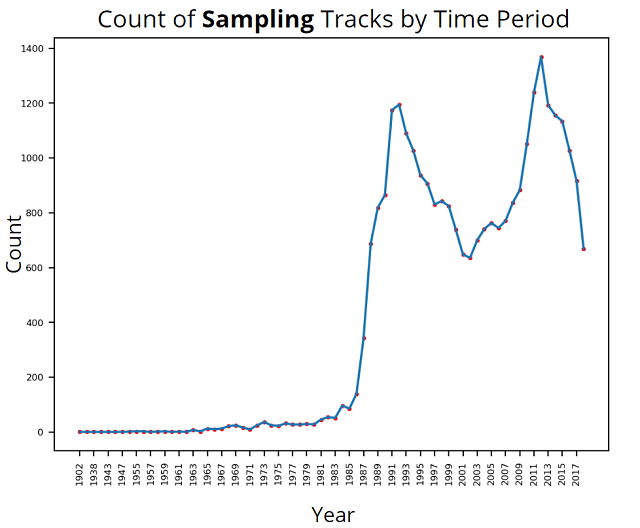
\includegraphics{TimePeriods/samplingTimePeriod}
\caption{Count of Sampling Tracks by Time Period}
\centering
\end{figure}
As seen in Figure xxx, sampling took a huge downturn from having up to ~1200 songs (out of the dataset) with samples in 1991 with an observably sharp downturn in sampling until 2001 when yearly sampling volume rose again.
\subsubsection{Does Hip-Hop sample music more often than other genres?}
Yes
\begin{figure}[H]
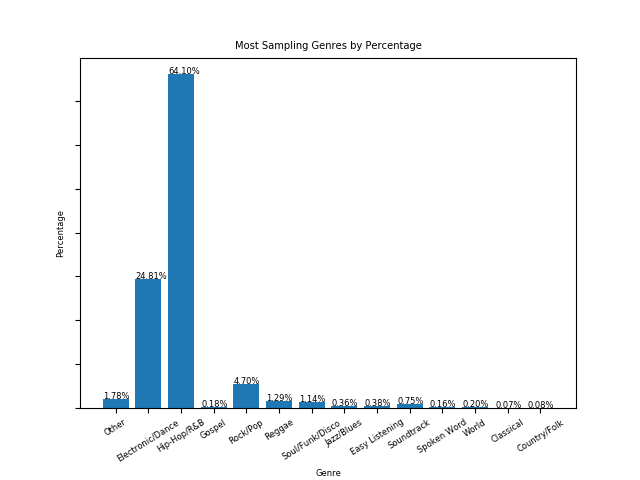
\includegraphics{topSamplingGenresPercent}
\caption{Most Sampling Genres Overall}
\centering
\end{figure}
\subsection{Most Influential Genres}
It's Soul/Funk/Disco
\begin{figure}[H]
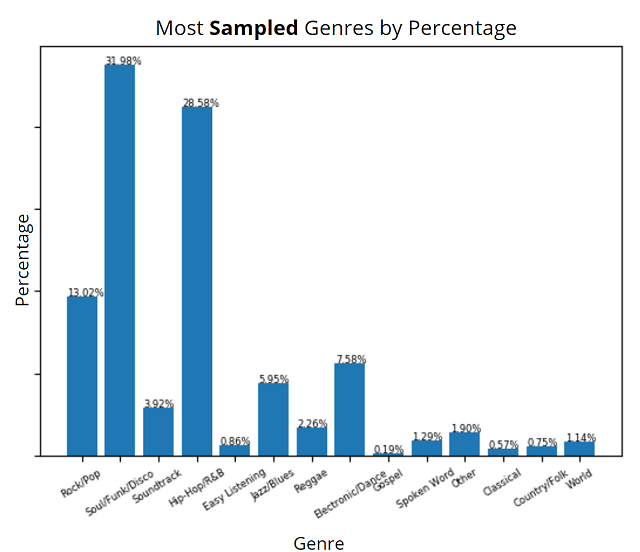
\includegraphics{topSampledGenresPercent}
\caption{Most Sampled Genres Overall}
\centering
\end{figure}
\subsection{Intra-genre and Inter-genre Sampling Strength}
Intra-genre sampling is a strong factor. 32.6\% of samples by artists are from other artists within their same genre.
\begin{figure}[H]
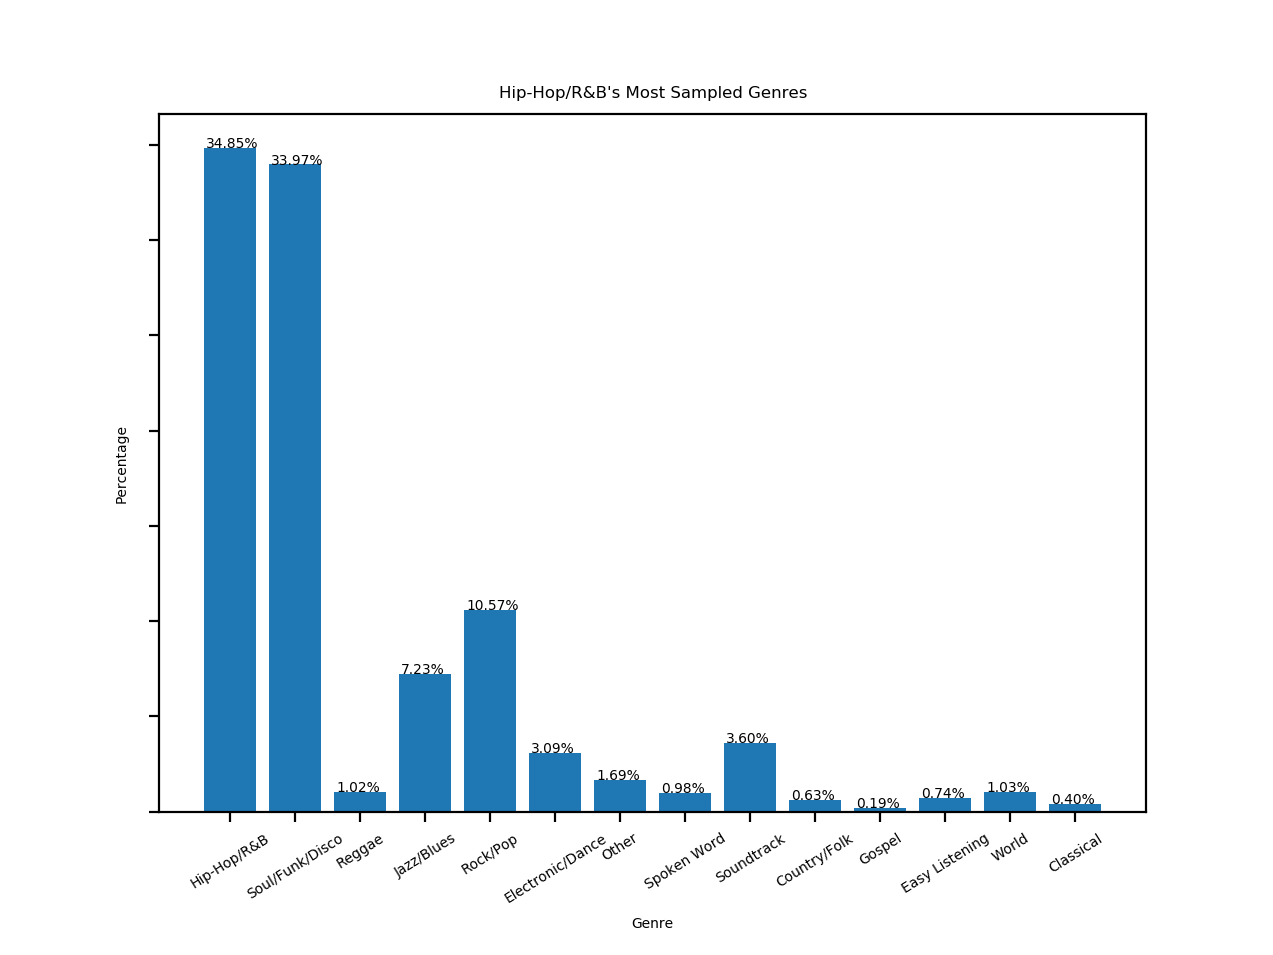
\includegraphics{./genreRatio/genreRatioHiphop}
\caption{Hip-Hop Sampling Proportions}
\centering
\end{figure}
\subsection{Patterns in Audio Element Sampling}
No patterns emerged
\begin{figure}[H]
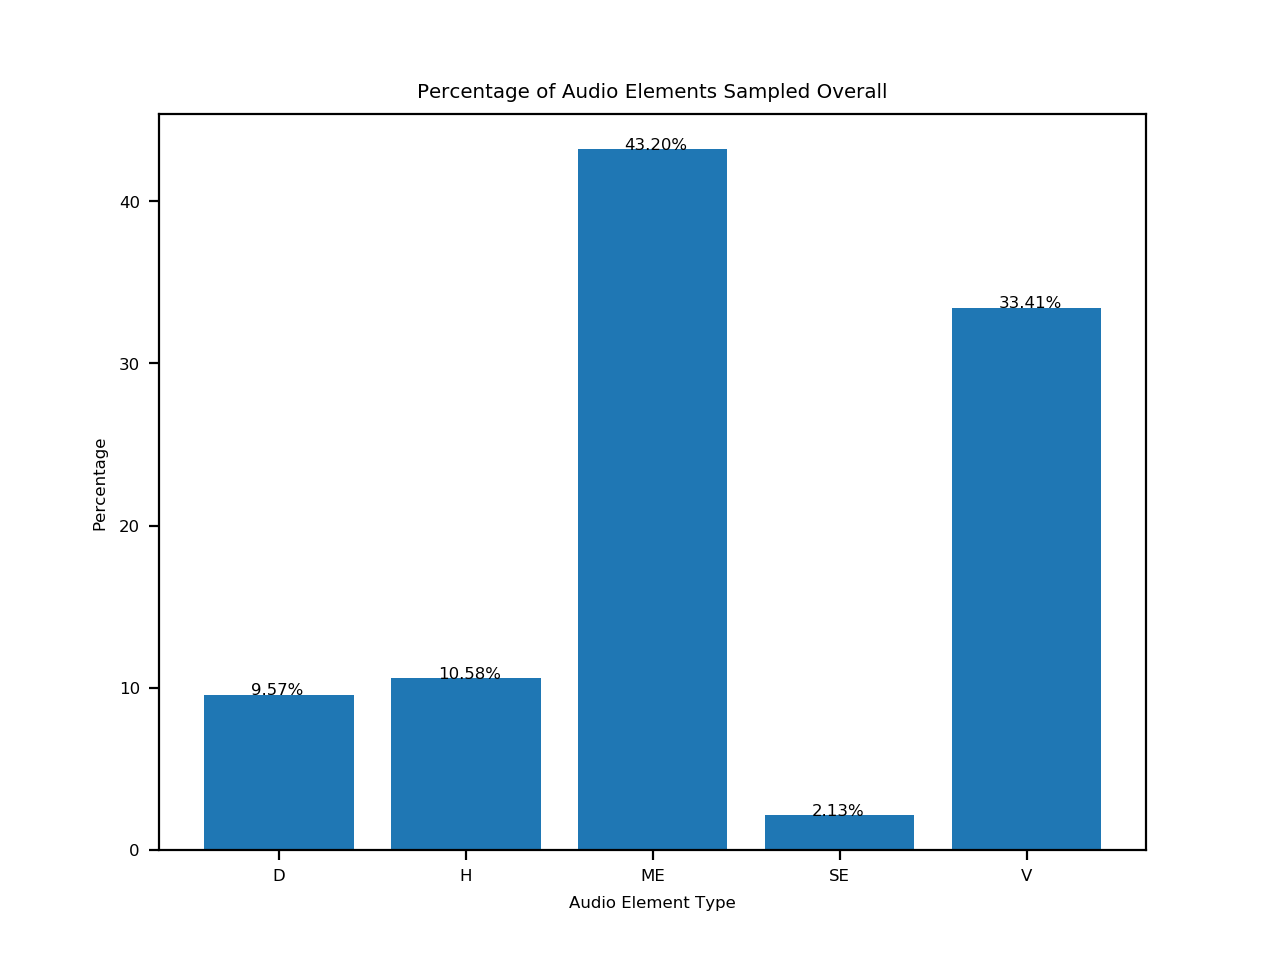
\includegraphics{audioElemSampledOverall}
\caption{Most Sampled Audio Elements Overall}
\centering
\end{figure}
But look at this ego graph of The Winstons where nearly all samplers only sample their drum break!
\begin{figure}[H]
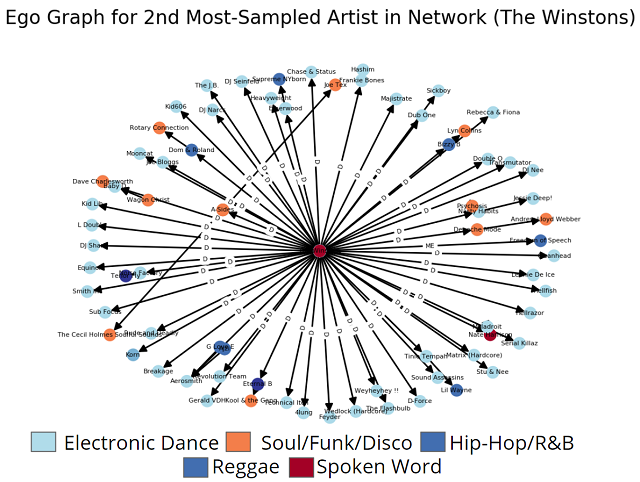
\includegraphics{./EgoGraphs/egoGraphMostSampled2TheWinstons}
\caption{The Winstons' Ego Graph}
\centering
\end{figure}
\subsection{Most Influential Artists}
\begin{table}[H]
\resizebox{\textwidth}{!}{%
\begin{tabular}{|l|l|l|l|l|l|l|}
\hline
\textbf{Rank} & \textbf{In-Degree Centrality} & \textbf{Betweenness Centrality} & \textbf{Closeness Centrality} & \textbf{Eigenvector Centrality} & \textbf{Katz Centrality} & \textbf{PageRank} \\ \hline
1. & James Brown & Public Enemy & James Brown & James Brown & James Brown & James Brown \\ \hline
2. & The Winstons & Beastie Boys & Lyn Collins & LL Cool J & Public Enemy & Lyn Collins \\ \hline
3. & Public Enemy & LL Cool J & The J.B.'s & Run-DMC & Lyn Collins & Afrika Bambaataa \\ \hline
4. & Lyn Collins & De La Soul & Fred Wesley & Lyn Collins & Run-DMC & Public Enemy \\ \hline
5. & Beside & Jay-Z & Beside & Public Enemy & LL Cool J & The Winstons \\ \hline
\end{tabular}%
}
\caption{Top Artist Centralities (All Time Periods)}
\end{table}
\begin{table}[H]
\resizebox{\textwidth}{!}{%
\begin{tabular}{|l|l|l|l|l|l|l|}
\hline
\textbf{Rank} & \textbf{In-Degree Centrality} & \textbf{Betweenness Centrality} & \textbf{Closeness Centrality} & \textbf{Eigenvector Centrality} & \textbf{Katz Centrality} & \textbf{PageRank} \\ \hline
1. & James Brown & Public Enemy & James Brown & James Brown & James Brown & James Brown \\ \hline
2. & Beside & Kurtis Blow & The J.B.'s & John Davis and the Monster Orchestra & Beside & Fred Wesley \\ \hline
3. & Run-DMC & Beastie Boys & Fred Wesley & Kurtis Blow & Run-DMC & The J.B.'s \\ \hline
4. & Public Enemy & Run-DMC & Beside & Run-DMC & Kurtis Blow & Afrika Bambaataa \\ \hline
5. & Kurtis Blow & James Brown & Afrika Bambaataa & The J.B.'s & Public Enemy & Beside \\ \hline
\end{tabular}%
}
\caption{Top Artist Centralities (1980's)}
\end{table}
\begin{table}[H]
\resizebox{\textwidth}{!}{%
\begin{tabular}{|l|l|l|l|l|l|l|}
\hline
\textbf{Rank} & \textbf{In-Degree Centrality} & \textbf{Betweenness Centrality} & \textbf{Closeness Centrality} & \textbf{Eigenvector Centrality} & \textbf{Katz Centrality} & \textbf{PageRank} \\ \hline
1. & James Brown & Public Enemy & James Brown & James Brown & James Brown & James Brown \\ \hline
2. & Public Enemy & Masta Ace Incorporated & Lyn Collins & Lyn Collins & Public Enemy & Lyn Collins \\ \hline
3. & The Winstons & LL Cool J & Fred Wesley & Fred Wesley & Lyn Collins & Fred Wesley \\ \hline
4. & Lyn Collins & Beastie Boys & Melvin Bliss & Parliament & N.W.A. & Public Enemy \\ \hline
5. & Run-DMC & De La Soul & Parliament & LL Cool J & Run-DMC & The Winstons \\ \hline
\end{tabular}%
}
\caption{Top Artist Centralities (1990's)}
\end{table}
\begin{table}[H]
\resizebox{\textwidth}{!}{%
\begin{tabular}{|l|l|l|l|l|l|l|}
\hline
\textbf{Rank} & \textbf{In-Degree Centrality} & \textbf{Betweenness Centrality} & \textbf{Closeness Centrality} & \textbf{Eigenvector Centrality} & \textbf{Katz Centrality} & \textbf{PageRank} \\ \hline
1. & James Brown & Jay-Z & The Notorious B.I.G. & The Notorious B.I.G. & The Notorious B.I.G. & Run-DMC \\ \hline
2. & The Winstons & Public Enemy & James Brown & Public Enemy & James Brown & Public Enemy \\ \hline
3. & The Notorious B.I.G. & Kanye West & Public Enemy & EPMD & Public Enemy & The Notorious B.I.G. \\ \hline
4. & Beside & 50 Cent & Beside & Run-DMC & Beside & James Brown \\ \hline
5. & Public Enemy & Nas & Run-DMC & James Brown & The Winstons & Beside \\ \hline
\end{tabular}%
}
\caption{Top Artist Centralities (2000's)}
\end{table}
\subsection{Louvain Communities}
\begin{table}[H]
\resizebox{\textwidth}{!}{%
\begin{tabular}{|l|l|l|l|l|l}
\cline{1-5}
\textbf{n'th Largest Louvain Community} & \multicolumn{4}{c|}{\textbf{Genre (\% in n'th Largest Community)}} &  \\ \cline{1-5}
\textbf{} & {\ul Hip-Hop/R\&B} & {\ul Electronic/Dance} & {\ul Rock/Pop} & {\ul Soul/Funk/Disco} &  \\ \cline{1-5}
1. & 55.56\% & 14.23\% & 10.35\% & 7.46\% &  \\ \cline{1-5}
2. & 59.68\% & 20.45\% & 5.56\% & 7.44\% &  \\ \cline{1-5}
3. & 56.84\% & 19.04\% & 6.64\% & 8.11\% &  \\ \cline{1-5}
4. & 55.57\% & 14.06\% & 7.29\% & 9.42\% &  \\ \cline{1-5}
5. & 12.20\% & 60.59\% & 8.71\% & 2.41\% &  \\ \cline{1-5}
\end{tabular}%
}
\caption{Top Genre Makeup in n'th Largest Louvain Communities}
\end{table}
The proportional makeup of each of the largest Louvain communities came to an unsurprising conclusion given our observations with intra-genre sampling: Each of the partitioned communities were dominated by a single genre.
\begin{figure}[H]
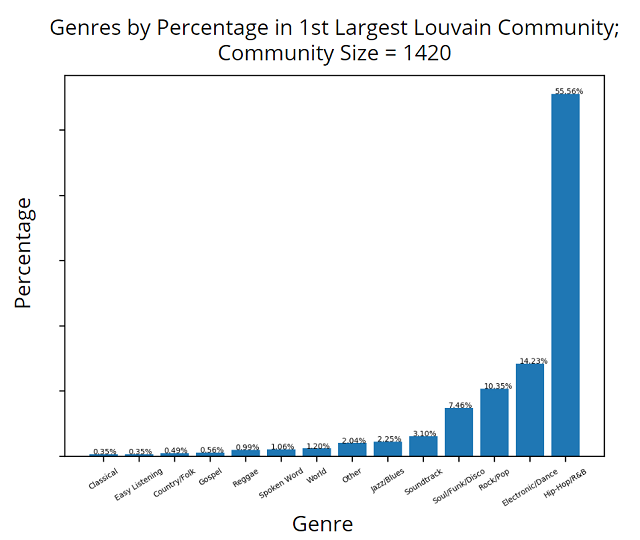
\includegraphics{LouvainCommunities/louvain1st}
\caption{Genre Makeup of Largest Louvain Community}
\centering
\end{figure}
As shown in Figure xxx, 55.56\% of artists in the largest Louvain Community are Hip-Hop/R\&B artists, indicating a high level of intra-level sampling and an insular sampling pattern. 
\section{Conclusion and Future Work}
\subsection{Conclusion}
\subsection{Future Work}
Future studies of musical sampling influence networks can look towards the patterns established by this paper to create an application capable of making predictions about the types of samples likely to be found in a song containing the specific defining characteristics we researched in this project. This predictive analysis could potentially aid developers such as WhoSampled with their music sampling identification software by acting as a false positive check.

From a legal perspective, the sampling patterns that establish the potential for a predictive algorithm could be used for ground truth facts during legal proceedings of musical sampling lawsuits. There are often initial arguments from parties debating whether a song was actually sampled by another song and a predictive algorithm could help determine the likelihood this is true based on an artist's past behaviors within the current musical community's trends.

Legal and historical scholars could also perform a deeper analysis of the dip in sampling volume post-1991 that is correlated with the Grand Upright Music v. Warner Bros. Records copyright case that famously ruled the specifics behind what constitutes a legal sample.
\section{Acknowledgments}
I would like to thank Professor Andrea LaPaugh for organizing the Network Analysis Independent Work seminar and advising this project. I would also like to thank Bobray J. Bordelon and Darwin F. Scott of the Princeton University Library for enabling access to the WhoSampled Academic Pro dataset.
\nocite{*}
\bstctlcite{bstctl:etal, bstctl:nodash, bstctl:simpurl}
\bibliographystyle{IEEEtranS}
\bibliography{references}

\end{document}